\chapter{Accuracy testing}
In order to show the accuracy of the methods and establish a meaningful use of (some of) the library's components, the following method was created.
\begin{figure}[h]
	\centering
	\begin{minipage}[b]{0.7\textwidth}
		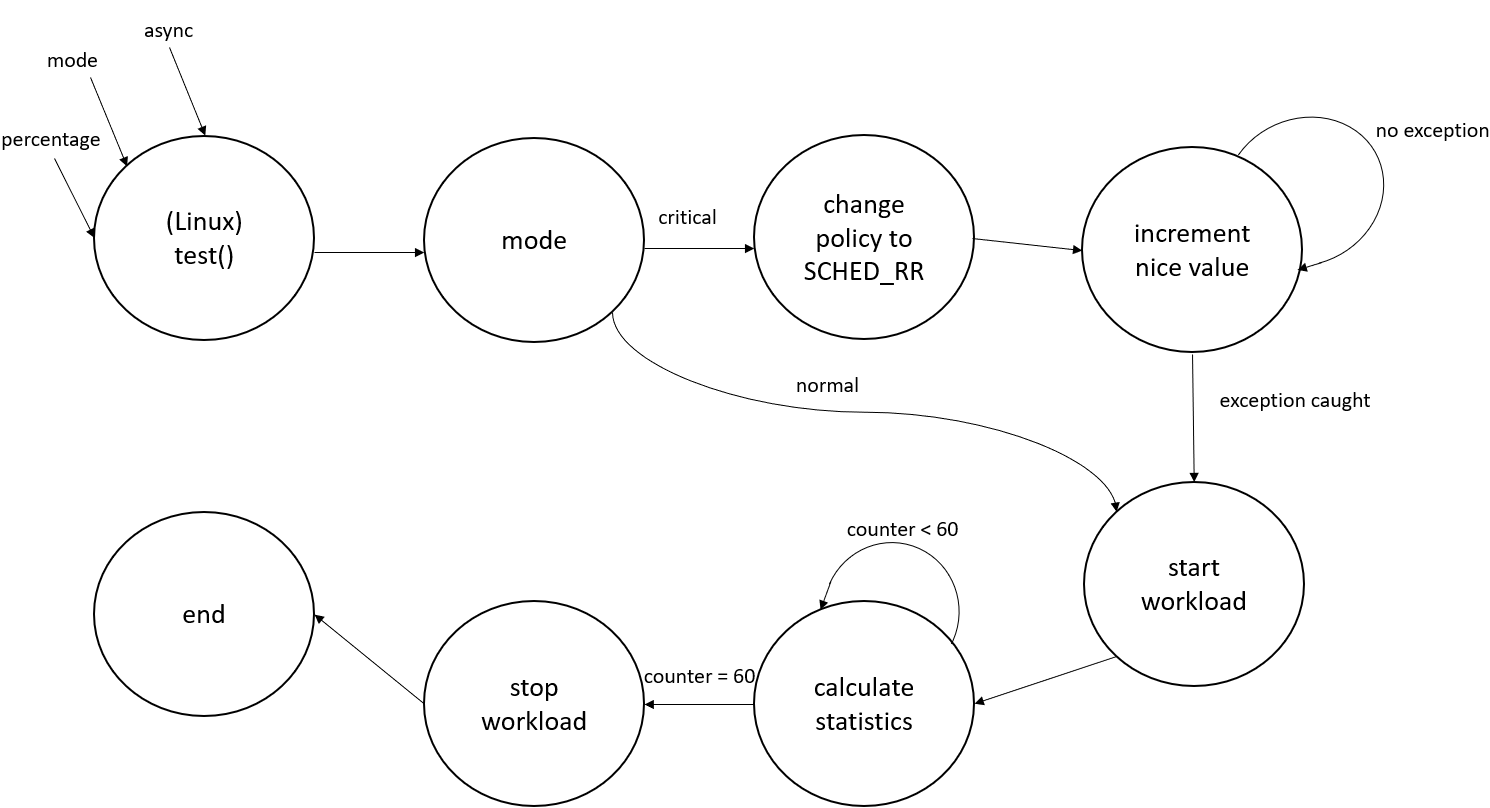
\includegraphics[width=\textwidth]{../figures/testing/test_linux.png}
		\caption{Testing method - Linux}
	\end{minipage}
	\begin{minipage}[b]{0.7\textwidth}
		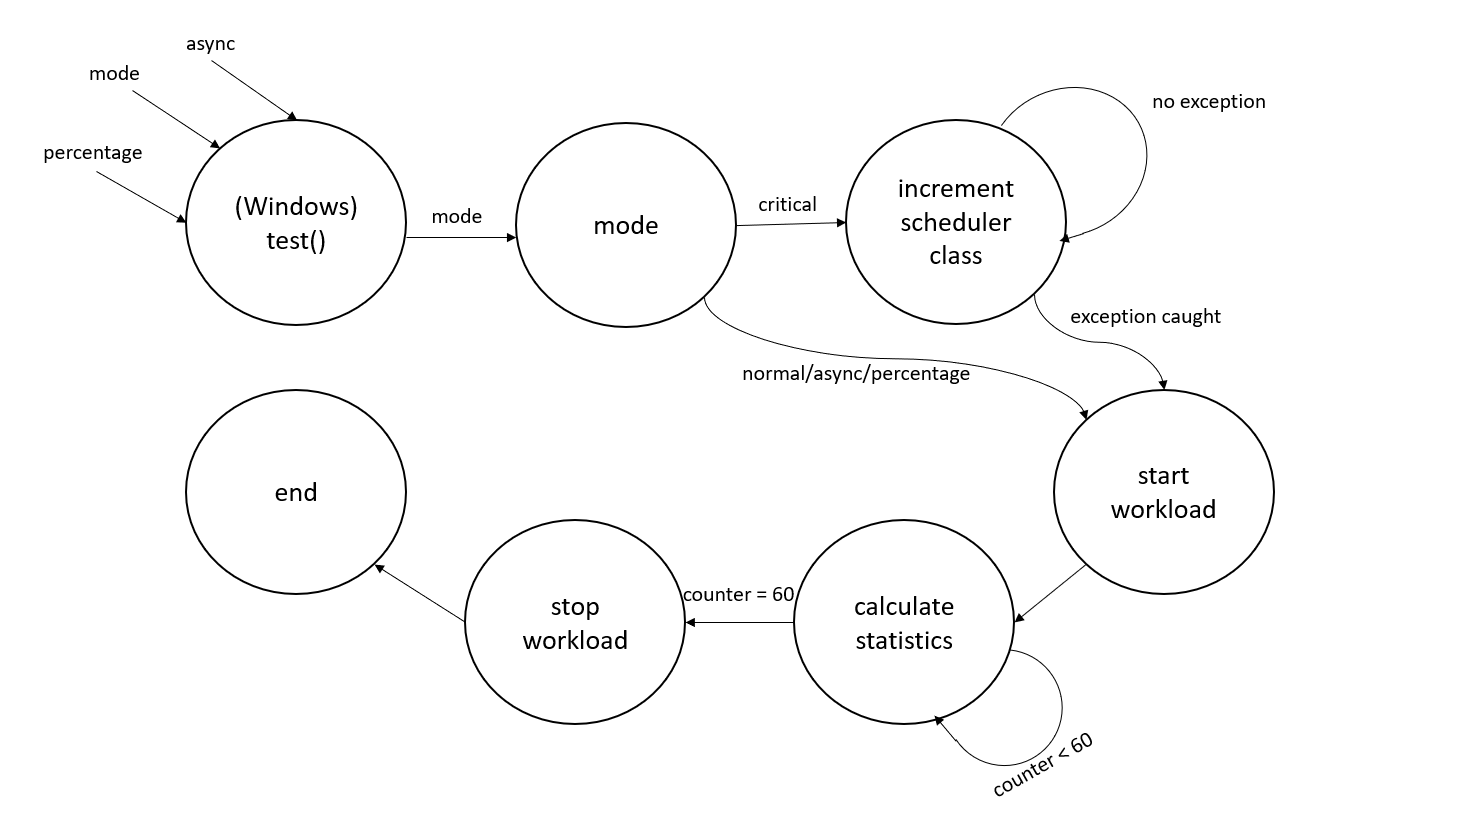
\includegraphics[width=\textwidth]{../figures/testing/test_windows.png}
		\caption{Testing method - Windows}
	\end{minipage}
\end{figure}\newpage
Here we pass the most crucial parameters:
\begin{enumerate}
	\item percentage: in order to specify how big the workload created should be 
	\item async: to verify if the asynchronous mode makes a huge impact on the system
	\item mode: which can be set either to \text{CRITICAL} (define that extends to one) or\\\textit{NORMAL} (define that extends to zero).
\end{enumerate}
The method first defines two lists that will contain the system's and process's workloads. Additionally it sets two flags to true to increase the process's priority (Linux: nice value / Windows: sched class) to maximum and a variable called \textit{prio} to null, which will later be set to \textit{MAX\_PRIO} (defined in \textit{workload.hpp}) to increase the priority of the workload's threads in case the mode was set to critical. The priority's incrementation is called in a \textit{try-catch} block. If this catches an exception we shall set the respective flags to false in order to avoid an endless loop.
Afterwards we create an object of type \textit{Workload} and we pass it the percentage, variable prio's reference and the asny argument. Then we start the workload and call \texttt{calculateAndShowLoad()} in order to see and get the system's statistics. Then we call \texttt{Workload.stopWL()} to stop the loops that create the artificial workload and \texttt{Workload.finishWorkload()} in order to also correctly terminate(join) the started workload threads. At last we use the \texttt{writeRuntimeStats()} function to write the statistics from the lists that we initialised at the begging of the test. This order is necessary for the user to get meaningful results. Small tests in the developing phase of this library showed that computers can't handle well a huge load and IO-operations at the same time. That's why the writing of two or more statistics needs to happen only after the workload was finished. 
 
The method can be called as followed:
\begin{figure}[!htbp]
	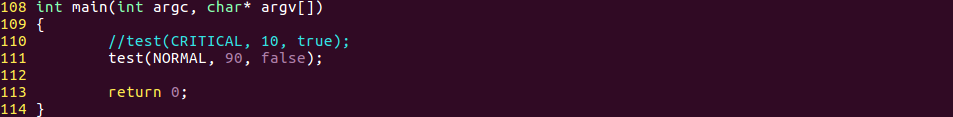
\includegraphics[width=\textwidth]{../figures/testing/main.png}
	\caption{Main testing method}
\end{figure}\\
To run the experiment the following steps were executed:\\
\begin{figure}[!htbp]
	\centering
	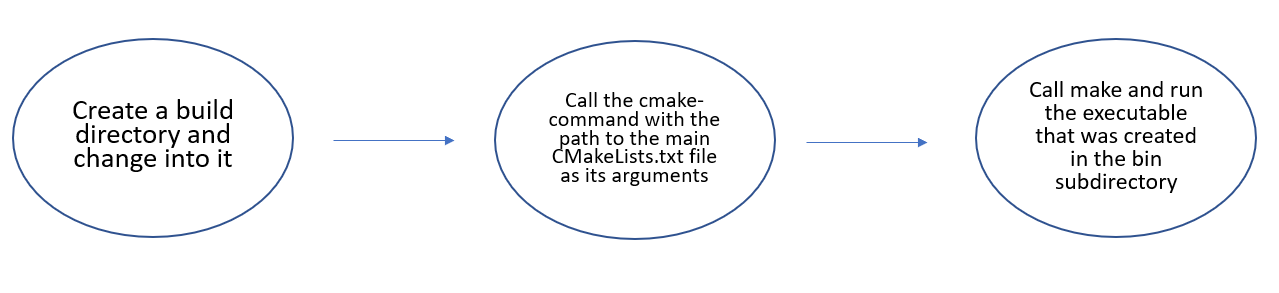
\includegraphics[scale=0.4]{../figures/testing/cmakeSteps.png}
	%\caption{Main testing method}
\end{figure}\\
This will create two log files:\textit{overall\_stats.csv} and \textit{runtime\_statistics.csv}.
\newpage
\section{Results}
\subsection{Linux}
The Linux machine under testing has the system's attributes and OS:
\begin{enumerate}
	\item OS: 				Ubuntu 16.04
	\item Processor: 		Intel Core i5-7200U, 2.50GHz
	\item Cores:			4
	\item Threads per Core:	2
	\item Architecture: 	x86\_64
\end{enumerate}
\subsubsection{Normal Mode}
Normal mode was tested with a 90\% workload. The results were as expected. Additionally the following statistics were logged in the \textit{overall\_stats.csv} file.
\begin{enumerate}
	\item Average System Workload: 90.2126
	\item Average Process Workload: 89.5858
	\item NIT\footnote{NotIdleTime}(time process was working out of 60 seconds): 60.00s 
\end{enumerate}  
\begin{figure}[!htbp]
	\centering
	\begin{minipage}[b]{\textwidth}
		\centering
		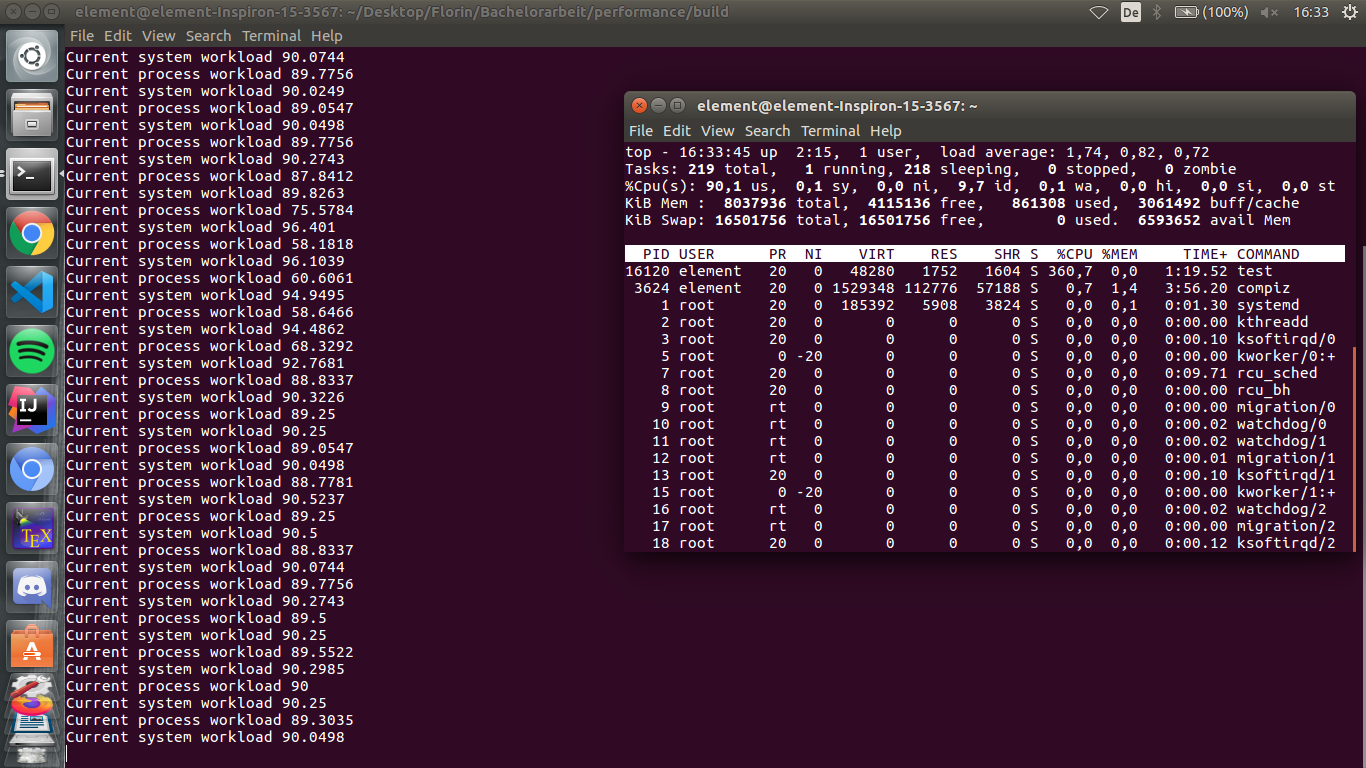
\includegraphics[scale=0.15]{../figures/testing/linux/normalStats/workload_normal.png}
		\caption{Library comparison with Linux's top-command: normal mode}
		\hspace{3mm}
	\end{minipage}
	\begin{minipage}[b]{\textwidth}
		\centering
		\includegraphics[scale=0.35]{../figures/testing/linux/normalStats/Stats.png}
		\caption{Overtime statistics: normal mode}
	\end{minipage}
\end{figure}
\newpage
\subsubsection{Critical Mode}
Critical mode was tested with a 10\% workload. The results were as expected. Additionally the following statistics were logged in the \textit{overall\_stats.csv} file.
\begin{enumerate}
	\item Average System Workload: 10.564
	\item Average Process Workload: 9.97427
	\item NIT(time process was working out of 60 seconds): 59.799s
\end{enumerate}
\begin{figure}[!htbp]
	\centering
	\begin{minipage}[b]{\textwidth}
		\centering
		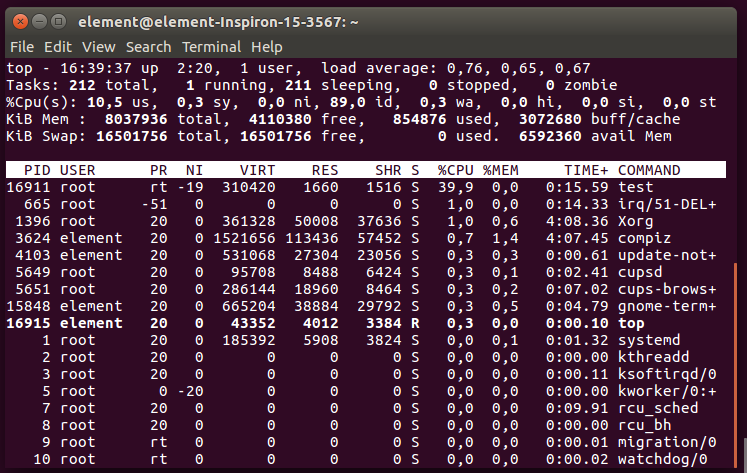
\includegraphics[scale=0.2]{../figures/testing/linux/criticalStats/workload_critical.png}
		\caption{Library comparison with Linux's top-command: normal mode}
		\hspace{3mm}
	\end{minipage}
	\begin{minipage}[b]{\textwidth}
		\centering
		\includegraphics[scale=0.6]{../figures/testing/linux/criticalStats/Stats.png}
		\caption{Overtime statistics: normal mode}
	\end{minipage}
\end{figure}
\newpage
\subsection{Windows}
The Windows machine under testing has the following system attributes and OS:
\begin{enumerate}
	\item OS: Microsoft Windows 10 Home
	\item Processor: Intel Core i7-8700, 3.20GHz
	\item Cores: 6
	\item Logical Cores: 12
	\item Architecture: x64-based-processor
\end{enumerate}
\subsubsection{Normal Mode}
As with Linux, normal mode was tested with a 90\% percent workload. The following values were logged in the comma separated files:
\begin{enumerate}
	\item Average System Workload: 87.8445
	\item Average Process Workload: 85.3584
	\item NIT: 66.040s
\end{enumerate}
\begin{figure}[!htbp]
	\centering
	\begin{minipage}[b]{\textwidth}
		\centering
		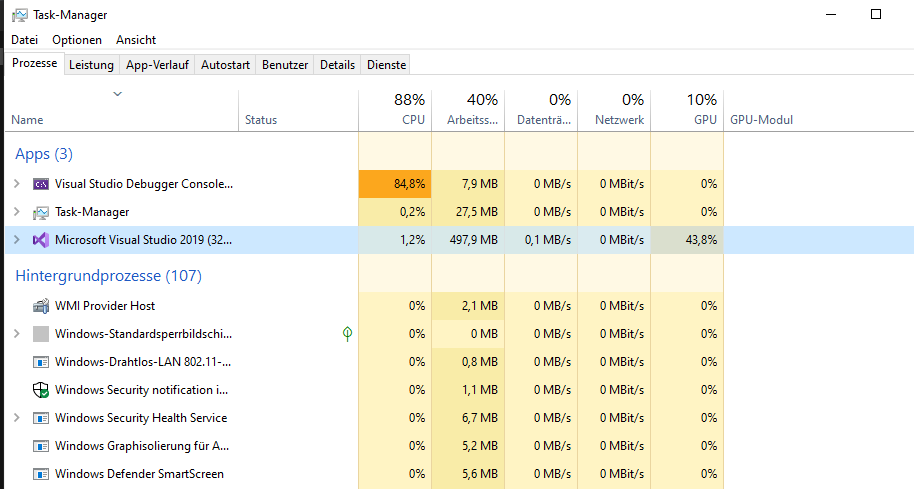
\includegraphics[scale=0.18]{../figures/testing/windows/normalStats/windows_normalMode.PNG}
		\caption{Library comparison with Windows's task manager: normal mode}
		\hspace{3mm}
	\end{minipage}
	\begin{minipage}[b]{\textwidth}
		\centering
		\includegraphics[scale=0.6]{../figures/testing/windows/normalStats/Stats.png}
		\caption{Overtime statistics: normal mode}
	\end{minipage}
\end{figure}


\newpage
\subsubsection{Critical Mode}
Critical mode was tested with a 10\% workload. The following values were logged in the comma separated files:
\begin{enumerate}
	\item Average System Workload: 10.351
	\item Average Process Workload: 8.22164
	\item NIT: 60.907s 
\end{enumerate}
\begin{figure}[!htbp]
	\centering
	\begin{minipage}[b]{\textwidth}
		\centering
		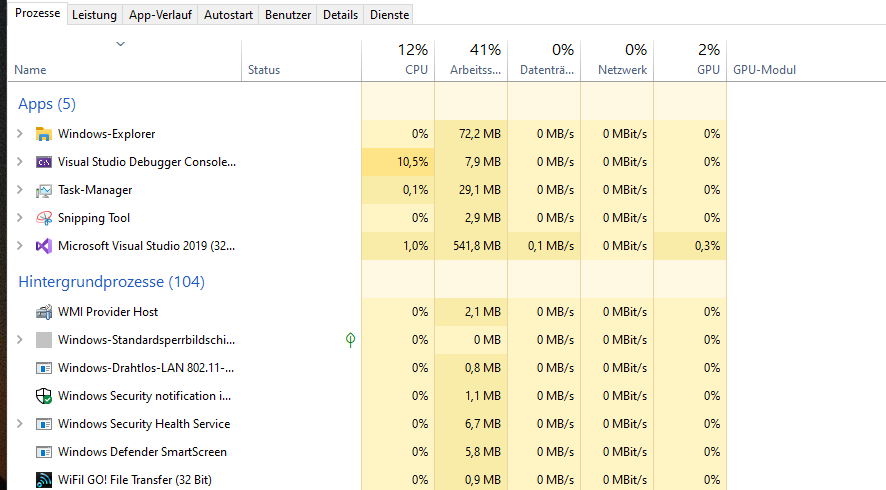
\includegraphics[scale=0.2]{../figures/testing/windows/criticalStats/Unbenannt.PNG}
		\caption{Library comparison with Windows's task manager: critical mode}
		\hspace{3mm}
	\end{minipage}
	\begin{minipage}[b]{\textwidth}
		\centering
		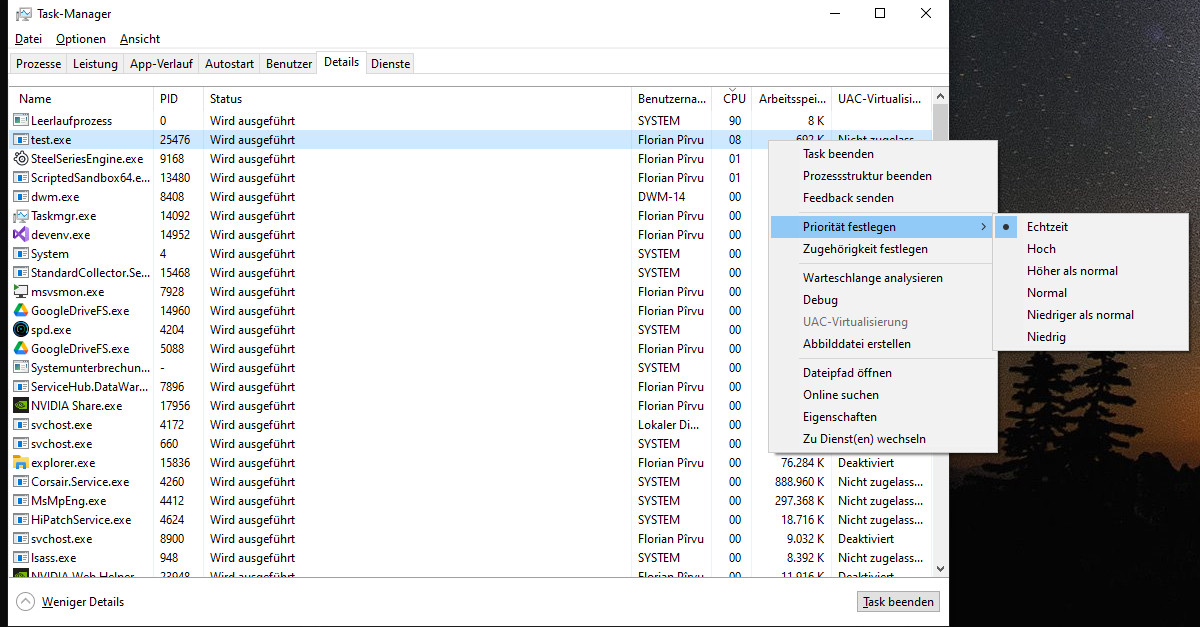
\includegraphics[scale=0.15]{../figures/testing/windows/criticalStats/priority.png}
		\caption{Task manager priority level}
		\hspace{3mm}
	\end{minipage}
	\begin{minipage}[b]{\textwidth}
		\centering
		\includegraphics[scale=0.6]{../figures/testing/windows/criticalStats/Stats.png}
		\caption{Overtime statistics: critical mode}
	\end{minipage}
\end{figure}
\newpage
\section{Findings}
\subsection{Linux}
Both critical and normal mode were successfully comparable to \textit{top\_command} pre-installed on every Unix machine. One can see that in normal more the process has a priority of 20 and a nice value of zero, which is standard on my Linux machine, while in critical mode the priority is set to \textit{RT}(which stands for real-time) and the nice value is -19 (the highest nice value on a Unix machine).\\
While testing the normal mode, one could observe the CPU's percentage exceeding the 100\% mark and reaching up to 360\%. This is due to the command adding each CPU's workload. Hence the result will show the number of CPUs that the machine has multiplied by the load that each CPU has. In our example we set the system's workload to 90\%. That means (in theory) each CPU will have to work 90 percent of the time, which results the load on the whole system would be:\vspace{1mm}\\
$number\_of\_CPUs(4) * workload(90\%) = top\_command\_display(360\%)$
\vspace{1mm}\\
This can also be seen in the critical mode test, where the system's workload was displayed as being almost 40\% when we set our workload to 10\%.\\
Additionally the expected system's workload remained in a reasonable range of $10 \pm 1.5\%$, while the process had a range of $10 \pm 1\%$ in the critical mode, while in normal mode the results are similar. Because of the low workload the process's NIT dropped a few milliseconds, which needs to be expected when the thread work only for 10\% of the time and for the rest 90\% they sleep.
\subsection{Windows}
On my Windows machine the results were resembling those on my Unix machine. The library's output was almost identical to that created by the \textit{task manager}. Similar to Linux the NIT on Windows also dropped a few milliseconds in critical mode. However the difference is substantial between the two operating systems. This might be because on Linux we also change the way the process is being scheduled, while on Windows we always use the same scheduler and increase only the priority of the test process. Besides that, the results can be considered satisfying. The workload's range and the process's priority have been pleasing.